\documentclass[color=blue,lang=cn,newtx,10pt,scheme=chinese]{elegantbook}

\title{数学物理方程习题集}
\subtitle{匠心之作}

\author{Huangchun Meng}
\institute{School of Mathematics NUAA}
\date{\today}
\version{1.0}

\extrainfo{注意:仅供参考,本人水平有限,若有错误,欢迎指正!}

\setcounter{tocdepth}{3}

\logo{logo-blue.png}
\cover{cover.jpg}

% 本文档命令
\usepackage{array}
\newcommand{\ccr}[1]{\makecell{{\color{#1}\rule{1cm}{1cm}}}}

% 修改标题页的橙色带
\definecolor{customcolor}{RGB}{32,178,170}
\colorlet{coverlinecolor}{customcolor}
\usepackage{cprotect}

\addbibresource[location=local]{reference.bib} % 参考文献,不要删除

\begin{document}

\maketitle
\frontmatter

\tableofcontents

\mainmatter

\chapter{数学物理方程简介}% Chapter 1

数学物理以研究物理问题为目标的数学理论和数学方法。它探讨物理现象的数学模型,即寻求物理现象的数学描述,
并对模型已确立的物理问题研究其数学解法,然后根据解答来诠释和预见物理现象,或者根据物理事实来修正原有模型。




\chapter{典型方程及其定解问题习题}% Chapter 2

\begin{introduction}
  \item 偏微分方程基本概念
  \item 弦振动方程(波动方程)
  \item 热传导方程(扩散方程)
  \item 位势方程(Laplace方程)
  \item 定解条件
  \item 初值问题
  \item 边值问题
  \item 定解问题适定性
\end{introduction}
\quad

\begin{exercise}
设有一长度为 $l$ 的均匀细杆,横截面为常数 $A$(图1-1),又设其侧面绝热,即热量只能沿长度方向传导,试推导杆的热传导方程.
\end{exercise}
\quad

\begin{solution}
  
\end{solution}
  
\quad

\begin{exercise}
对练习2.1中的均匀细杆,其初始温度为 $\phi (x)$,两端满足下列边界条件:

(1)一端绝热,另一端保持常温 $u_0$;

(2)两端分别有恒定的密度 $q_1$ 和 $q_2$ 的热量进入;

(3)一端温度为 $\mu (t)$,另一端与温度为 $Q(t)$ 的介质有热交换.

试分别写出这三种热传导过程的定解问题.
\end{exercise}
\quad

\begin{solution}
  
\end{solution}
\quad

\begin{exercise}
有一圆锥形轴(图1-2),其高为 $h$,密度和杨氏模量分别为常数 $\rho$ 和 $E$,试证明其纵振动方程为
\begin{equation}
  E\frac{\partial}{\partial x}[(1-\frac{x}{h})^2\frac{\partial u}{\partial x}]=\rho (1-\frac{x}{h})^2\frac{\partial^2 u}{\partial t^2}
\end{equation}
\end{exercise}
\quad

\begin{proof}
  
\end{proof}
\quad




\chapter{二阶线性偏微分方程的分类与化简习题}% Chapter 3

\begin{introduction}
  \item 两个自变量的二阶线性偏微分方程
  \item 多个自变量的二阶线性偏微分方程
  \item 方程的分类
  \item 椭圆形
  \item 抛物形
  \item 双曲形
  \item 方程的化简
  \item 标准型
\end{introduction}
\quad

\begin{exercise}
判定下列方程的类型:

(1) $x^2u_{xx}-y^2u_{yy}=0$;

(2) $u_{xx}+(x+y)^2u_{yy}=0$.
\end{exercise}
\quad

\begin{solution}
  
\end{solution}
\quad

\begin{exercise}
化下列方程为标准型:

(1) $u_{xx}+4u_{xy}+5u_{yy}+u_x+u_y=0$;

(2) $u_{xx}-4u_{xy}+u_{yy}=0$.
\end{exercise}
\quad

\begin{solution}
  
\end{solution}
\quad

\begin{exercise}
判定下列方程类型:

(1) $u_{xx}+2u_{xt}-u_{tt}=0$;

(2) $k^2u_{xx}+(1+k^2)u_{yy}-k^2u_t=0$ (k为常数).
\end{exercise}
\quad

\begin{solution}
  
\end{solution}
\quad




\chapter{分离变量法习题}% Chapter 4

\begin{introduction}
  \item 分离变量法
  \item 固有值问题(Sturm-Liouville问题)
  \item 解的存在性
  \item 齐次化原理(Duhamel原理)
  \item 固有函数展开(Fourier级数展开)
  \item 边界条件齐次化
\end{introduction}
\quad

\begin{exercise}
  解下列定解问题:

  $\begin{cases}
    u_t=a^2u_{xx}, & 0<x<l,\ t>0,\\
    u|_{t=0} =\phi (x), & 0\leq x\leq l,\\
    u_x|_{x=0}=0,u_x|_{x=l}=0, & t\geq 0.
  \end{cases}$
\end{exercise}
\quad

\begin{solution}

\end{solution}
\quad

\begin{exercise}
  解下列定解问题:

  (1) $\begin{cases}
    u_{tt}=a^2u_{xx}+f(x,t), & 0<x<l,\ t>0,\\
    u|_{t=0} =\phi (x),u_t|_{t=0}=\psi (x), & 0\leq x\leq l,\\
    u_x|_{x=0}=0,u|_{x=l}=0, & t\geq 0.
  \end{cases}$
  
  \quad
  
  (2) $\begin{cases}
    u_{tt}=a^2u_{xx}, & 0<x<1,\ t>0,\\
    u|_{t=0}=
    \begin{cases}
      x, & 0\leq x\leq \frac{1}{2},\\
      1-x, & \frac{1}{2}<x\leq 1,
    \end{cases}\\
    u_t|_{t=0}=x(1-x), & 0\leq x\leq 1,\\
    u|_{x=0}=u|_{x=1}=0, & t\geq 0.
    \end{cases}$
\end{exercise}
\quad

\begin{solution}
  
\end{solution}



\chapter{ElegantBook 写作示例}% Chapter

\begin{introduction}
  \item 积分定义~\ref{def:int}
  \item Fubini 定理~\ref{thm:fubi}
  \item 最优性原理~\ref{pro:max}
  \item 柯西列性质~\ref{property:cauchy}
  \item 韦达定理
\end{introduction}

\section{Lebesgue 积分}
在前面各章做了必要的准备后,本章开始介绍新的积分。在 Lebesgue 测度理论的基础上建立了 Lebesgue 积分,其被积函数和积分域更一般,可以对有界函数和无界函数统一处理。正是由于 Lebesgue 积分的这些特点,使得 Lebesgue 积分比 Riemann 积分具有在更一般条件下的极限定理和累次积分交换积分顺序的定理,这使得 Lebesgue 积分不仅在理论上更完善,而且在计算上更灵活有效。

Lebesgue 积分有几种不同的定义方式。我们将采用逐步定义非负简单函数,非负可测函数和一般可测函数积分的方式。

由于现代数学的许多分支如概率论、泛函分析、调和分析等常常用到一般空间上的测度与积分理论,在本章最后一节将介绍一般的测度空间上的积分。

\subsection{积分的定义}

我们将通过三个步骤定义可测函数的积分。首先定义非负简单函数的积分。以下设 $E$ 是 $\mathcal{R}^n$ 中的可测集。

\begin{definition}[可积性] \label{def:int} 
设 $ f(x)=\sum\limits_{i=1}^{k} a_i \chi_{A_i}(x)$ 是 $E$ 上的\textbf{非负简单函数},中文其中 $\{A_1,A_2,\ldots,A_k\}$ 是 $E$ 上的一个可测分割,$a_1,a_2,\ldots,a_k$ 是非负实数。定义 $f$ 在 $E$ 上的积分为 $\int_{a}^b f(x)$
\begin{equation}
   \label{inter}
   \int_{E} f dx = \sum_{i=1}^k a_i m(A_i) \pi \alpha\beta\sigma\gamma\nu\xi\epsilon\varepsilon. \oint_{a}^b\ointop_{a}^b\prod_{i=1}^n
\end{equation}
一般情况下 $0 \leq \int_{E} f dx \leq \infty$。若 $\int_{E} f dx < \infty$,则称 $f$ 在 $E$ 上可积。
\end{definition}

一个自然的问题是,Lebesgue 积分与我们所熟悉的 Riemann 积分有什么联系和区别?在 4.4 在我们将详细讨论 Riemann 积分与 Lebesgue 积分的关系。这里只看一个简单的例子。设 $D(x)$ 是区间 $[0,1]$ 上的 Dirichlet 函数。即 $D(x)=\chi_{Q_0}(x)$,其中 $Q_0$ 表示 $[0,1]$ 中的有理数的全体。根据非负简单函数积分的定义,$D(x)$ 在 $[0,1]$ 上的 Lebesgue 积分为
\begin{equation}
   \label{inter2}
   \int_0^1 D(x)dx = \int_0^1 \chi_{Q_0} (x) dx = m(Q_0) = 0
\end{equation}
即 $D(x)$ 在 $[0,1]$ 上是 Lebesgue 可积的并且积分值为零。但 $D(x)$ 在 $[0,1]$ 上不是 Riemann 可积的。


有界变差函数是与单调函数有密切联系的一类函数。有界变差函数可以表示为两个单调递增函数之差。与单调函数一样,有界变差函数几乎处处可导。与单调函数不同,有界变差函数类对线性运算是封闭的,它们构成一线空间。练习题 \ref{exer:43} 是一个性质的证明。

\begin{exercise}\label{exer:43}
设 $f \notin\in L(\mathcal{R}^1)$,$g$ 是 $\mathcal{R}^1$ 上的有界可测函数。证明函数
\begin{equation}
   \label{ex:1}
   I(t) = \int_{\mathcal{R}^1} f(x+t)g(x)dx \quad t \in \mathcal{R}^1
\end{equation}
是 $\mathcal{R}^1$ 上的连续函数。 
\end{exercise}

\begin{solution}
即 $D(x)$ 在 $[0,1]$ 上是 Lebesgue 可积的并且积分值为零。但 $D(x)$ 在 $[0,1]$ 上不是 Riemann 可积的。
\end{solution}

\begin{proof}
即 $D(x)$ 在 $[0,1]$ 上是 Lebesgue 可积的并且积分值为零。但 $D(x)$ 在 $[0,1]$ 上不是 Riemann 可积的。
\end{proof}

\begin{theorem}[Fubini 定理] \label{thm:fubi} 
(1)若 $f(x,y)$ 是 $\mathcal{R}^p\times\mathcal{R}^q$ 上的非负可测函数,则对几乎处处的 $x\in \mathcal{R}^p$,$f(x,y)$ 作为 $y$ 的函数是 $\mathcal{R}^q$ 上的非负可测函数,$g(x)=\int_{\mathcal{R}^q}f(x,y) dy$ 是 $\mathcal{R}^p$ 上的非负可测函数。并且
\begin{equation}
   \label{eq:461}
   \int_{\mathcal{R}^p\times\mathcal{R}^q} f(x,y) dxdy=\int_{\mathcal{R}^p}\left(\int_{\mathcal{R}^q}f(x,y)dy\right)dx.
\end{equation}

(2)若 $f(x,y)$ 是 $\mathcal{R}^p\times\mathcal{R}^q$ 上的可积函数,则对几乎处处的 $x\in\mathcal{R}^p$,$f(x,y)$ 作为 $y$ 的函数是 $\mathcal{R}^q$ 上的可积函数,并且 $g(x)=\int_{\mathcal{R}^q}f(x,y) dy$ 是 $\mathcal{R}^p$ 上的可积函数。而且~\eqref{eq:461} 成立。
\end{theorem}

\begin{note}
在本模板中,引理(lemma),推论(corollary)的样式和定理~\ref{thm:fubi} 的样式一致,包括颜色,仅仅只有计数器的设置不一样。
\end{note}

我们说一个实变或者复变量的实值或者复值函数是在区间上平方可积的,如果其绝对值的平方在该区间上的积分是有限的。所有在勒贝格积分意义下平方可积的可测函数构成一个希尔伯特空间,也就是所谓的 $L^2$ 空间,几乎处处相等的函数归为同一等价类。形式上,$L^2$ 是平方可积函数的空间和几乎处处为 0 的函数空间的商空间。

\begin{proposition}[最优性原理] \label{pro:max}
如果 $u^*$ 在 $[s,T]$ 上为最优解,则 $u^*$ 在 $[s, T]$ 任意子区间都是最优解,假设区间为 $[t_0, t_1]$ 的最优解为 $u^*$ ,则 $u(t_0)=u^{*}(t_0)$,即初始条件必须还是在 $u^*$ 上。
\end{proposition}

我们知道最小二乘法可以用来处理一组数据,可以从一组测定的数据中寻求变量之间的依赖关系,这种函数关系称为经验公式。本课题将介绍最小二乘法的精确定义及如何寻求点与点之间近似成线性关系时的经验公式。假定实验测得变量之间的 $n$ 个数据,则在平面上,可以得到 $n$ 个点,这种图形称为 “散点图”,从图中可以粗略看出这些点大致散落在某直线近旁, 我们认为其近似为一线性函数,下面介绍求解步骤。

\begin{figure}[htbp]
  \centering
  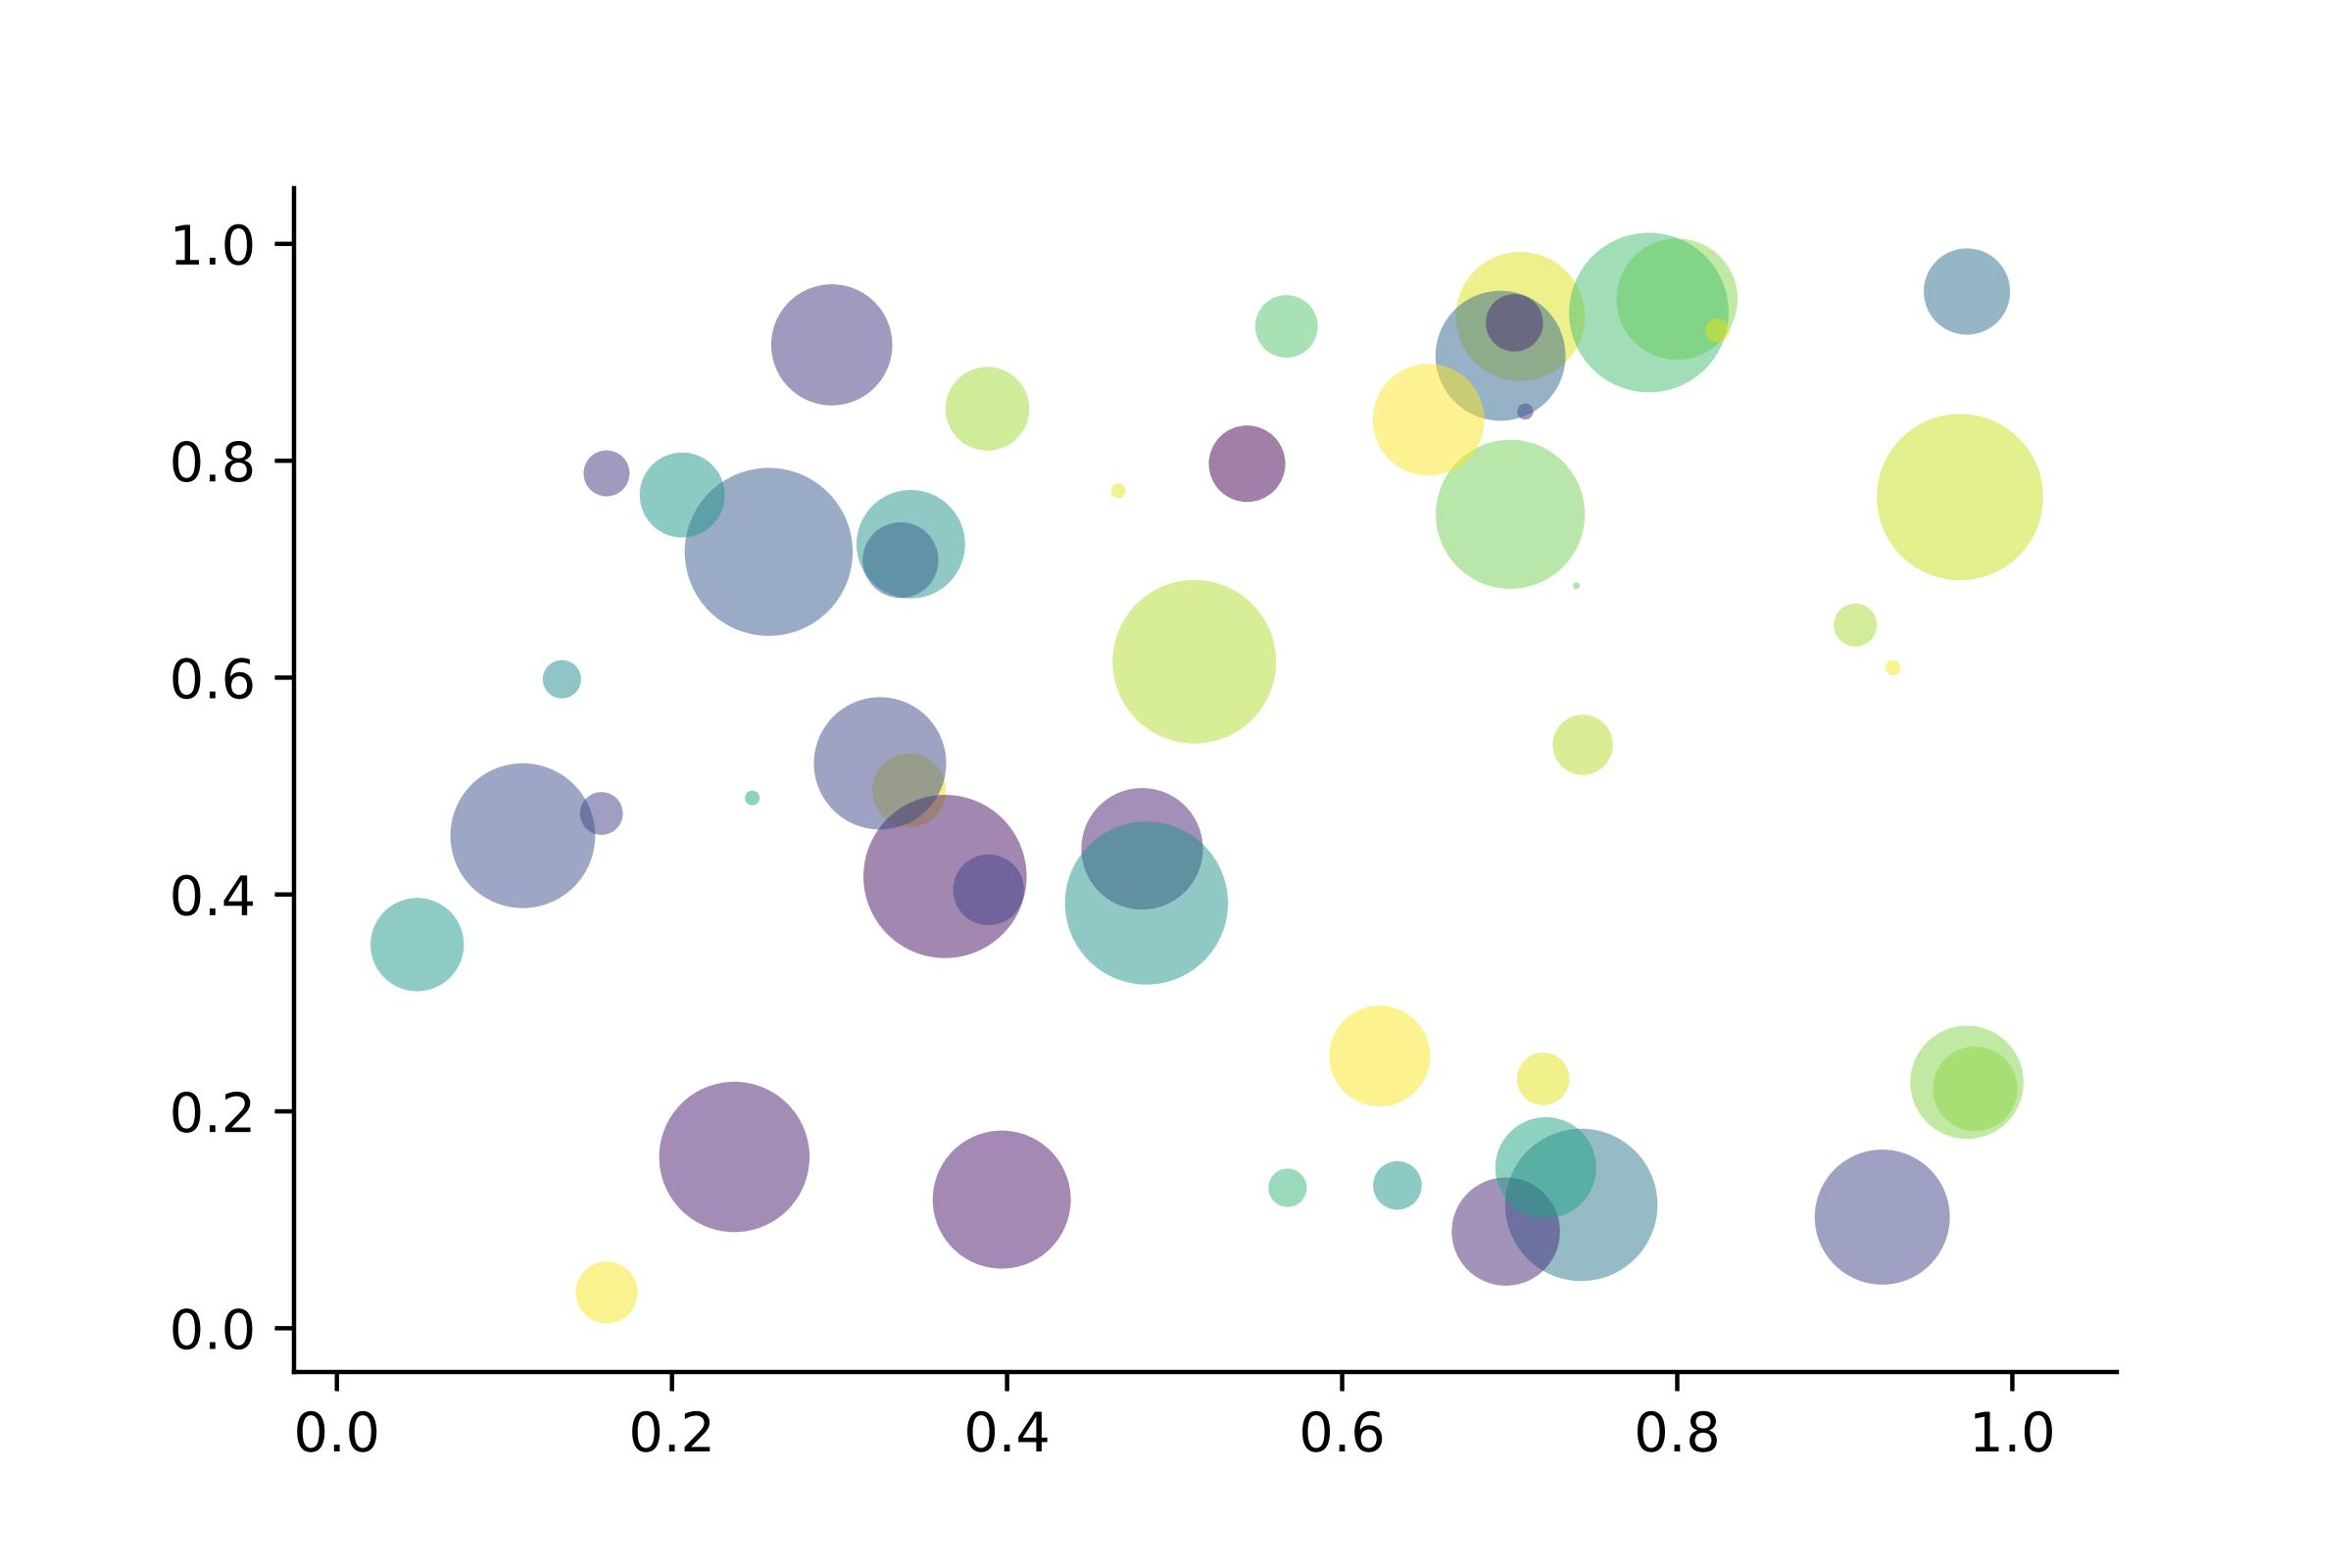
\includegraphics[width=0.6\textwidth]{scatter.jpg}
  \caption{散点图示例 $\hat{y}=a+bx$ \label{fig:scatter}}
\end{figure}

以最简单的一元线性模型来解释最小二乘法。什么是一元线性模型呢?监督学习中,如果预测的变量是离散的,我们称其为分类(如决策树,支持向量机等),如果预测的变量是连续的,我们称其为回归。回归分析中,如果只包括一个自变量和一个因变量,且二者的关系可用一条直线近似表示,这种回归分析称为一元线性回归分析。如果回归分析中包括两个或两个以上的自变量,且因变量和自变量之间是线性关系,则称为多元线性回归分析。对于二维空间线性是一条直线;对于三维空间线性是一个平面,对于多维空间线性是一个超平面。

\begin{property}\label{property:cauchy}
柯西列的性质
\begin{enumerate}
\item $\{x_k\}$ 是柯西列,则其子列 $\{x_k^i\}$ 也是柯西列。
\item $x_k\in \mathcal{R}^n$,$\rho(x,y)$ 是欧几里得空间,则柯西列收敛,$(\mathcal{R}^n,\rho)$ 空间是完备的。
\end{enumerate}
\end{property}

\begin{conclusion}
回归分析(regression analysis) 是确定两种或两种以上变量间相互依赖的定量关系的一种统计分析方法。运用十分广泛,回归分析按照涉及的变量的多少,分为一元回归和多元回归分析;按照因变量的多少,可分为简单回归分析和多重回归分析;按照自变量和因变量之间的关系类型,可分为线性回归分析和非线性回归分析。
\end{conclusion}

\begin{problemset}
\item 设 $A$ 为数域 $K$ 上的 $n$ 级矩阵。证明:如果 $K^n$ 中任意非零列向量都是 $A$ 的特征向量,则 $A$ 一定是数量矩阵。
\item 证明:不为零矩阵的幂零矩阵不能对角化。
\item 设 $A = (a_{ij})$ 是数域 $K$ 上的一个 $n$ 级上三角矩阵,证明:如果 $a_{11} = a_{22} = \cdots = a_{nn}$,并且至少有一个 $a_{kl} \not = 0 (k < l)$,则 $A$ 一定不能对角化。
\end{problemset}



\nocite{*}

\printbibliography[heading=bibintoc, title=\ebibname]
\appendix

\chapter{基本数学工具}


本附录包括了计量经济学中用到的一些基本数学,我们扼要论述了求和算子的各种性质,研究了线性和某些非线性方程的性质,并复习了比例和百分数。我们还介绍了一些在应用计量经济学中常见的特殊函数,包括二次函数和自然对数,前 4 节只要求基本的代数技巧,第 5 节则对微分学进行了简要回顾;虽然要理解本书的大部分内容,微积分并非必需,但在一些章末附录和第 3 篇某些高深专题中,我们还是用到了微积分。

\section{求和算子与描述统计量}

\textbf{求和算子} 是用以表达多个数求和运算的一个缩略符号,它在统计学和计量经济学分析中扮演着重要作用。如果 $\{x_i: i=1, 2, \ldots, n\}$ 表示 $n$ 个数的一个序列,那么我们就把这 $n$ 个数的和写为:

\begin{equation}
\sum_{i=1}^n x_i \equiv x_1 + x_2 +\cdots + x_n
\end{equation}



\end{document}
